
\de{ĐỀ THI GIỮA HỌC KỲ II NĂM HỌC 2022-2023}{THPT Trần Khai Nguyên}

\begin{bt}%[0T7B2-1]%[Dự án đề kiểm tra GKII NH22-23- Hiếu Phan]%[THPT Trần Khai Nguyên]
	Giải bất phương trình $ 4x^2+5x>x(x-3) -5$.
\loigiai{
    Ta có $ 4x^2+5x>x(x-3) -5 \Leftrightarrow 3x^2+8x+5>0$.\\
    BXD% Cần khai báo \usepackage{tkz-tab}
  \begin{center}
        \begin{tikzpicture}
        \tkzTabInit[nocadre=false,lgt=3,espcl=2,deltacl=0.5]{$x$/1 ,$3x^2+8x+5$/1}
        {$-\infty$ , $-\dfrac{5}{3}$ , $-1$ , $+\infty$}
        \tkzTabLine{, + , z , - , z , + }
    \end{tikzpicture}
  \end{center}
Dựa vào BXD ta suy ra bất phương trình có tập nghiệm $ S=\left(-\infty; -\dfrac{5}{3}\right) \cup (-1;+\infty)$.
}

\end{bt}
\begin{bt}%[0T7K3-2]%[Dự án đề kiểm tra GKII NH22-23- Hiếu Phan]%[THPT Trần Khai Nguyên]
    Giải phương trình $ \sqrt{2x^2+3x-5}=x+1$.
    \loigiai{
    Bình phương  hai vế phương trình  $2 \sqrt{2x^2+3x-5}=x+1\quad(*)$, ta được 
    \begin{eqnarray*}
        &&\sqrt{2x^2+3x-5}=x+1\\
        &\Rightarrow& 2x^2+3x-5 =x^2+2 x+1\\
        &\Leftrightarrow& x^2+x-6=0\\
        &\Leftrightarrow&\hoac{& x=-3\\ & x=2.}
    \end{eqnarray*}
    Thử lại
    \begin{itemize}
        \item Với $x=-3$, thay vào $(*)$ không thoả nên $x=-3$ loại.
        \item Với $x=2$, thay vào $(*)$ thoả nên $x=2$ nhận.
    \end{itemize}
    Vậy tập nghiệm của phương trình là $S=\left\lbrace 2 \right\rbrace$.
}
\end{bt}
\begin{bt}%[0T7K2-1]%[Dự án đề kiểm tra GKII NH22-23- Hiếu Phan]%[THPT Trần Khai Nguyên]
   Một mảnh vườn hình chữ nhật có chu vi $ 42 $ cm. Biết diện tích của mảnh vườn ít nhất là $ 108~\mathrm{cm^2} $. Hỏi chiều dài của mảnh vườn nằm trong khoảng nào?
    \loigiai{
    Gọi chiều dài của mảnh vườn hình chữ nhật là $ x (x>0)$ cm  .\\
    Khi đó chiều rộng của mảnh vườn là $ 21-x $ cm.\\
    Diện tích của mảnh vườn ít nhất là $ 108~\mathrm{cm^2} $ nên suy ra
    $$ x(21-x)\le 108 \Leftrightarrow -x^2+21x-108\le  0\Leftrightarrow 9\le x \le 12.$$
    Vậy chiều dài của mảnh vườn nằm trong khoảng từ $ 9 $ cm đến $ 12 $ cm.
}
\end{bt}

\begin{bt}%[0T8Y1-2]%[Dự án đề kiểm tra giữa HKII NH22-23- Nguyễn Sĩ Đạt]%[THPT Trần Khai Nguyên]
	Trường trung học phổ thông Trần Khai Nguyên có đội tuyển học sinh giỏi Toán lớp $12$ gồm $5$ học sinh, đội tuyển học sinh giỏi giải Toán trên máy tính cầm tay lớp $12$ có $10$ học sinh. Câu lạc bộ Toán \lq\lq Math - soul of life\rq\rq\ tổ chức buổi sinh hoạt giao lưu, muốn mời mỗi đội tuyển một thành viên đến để chia sẻ phương pháp học tập. Hỏi có bao nhiêu cách để lựa chọn hai học sinh thuộc hai đội tuyển trên?
	\loigiai
	{
		Chọn một học sinh từ đội tuyển học sinh giỏi Toán lớp $12$ có $5$ cách.\\
		Chọn một học sinh từ đội tuyển học sinh giỏi giải Toán trên máy tính cầm tay lớp $12$ có $10$ cách.\\
		Vậy có $5\cdot 10=50$ cách chọn thỏa mãn đề bài.
	}
\end{bt}

\begin{bt}%[0T8B1-3]%[Dự án đề kiểm tra giữa HKII NH22-23- Nguyễn Sĩ Đạt]%[THPT Trần Khai Nguyên]
	Từ các chữ số $0$, $1$, $2$, $3$, $4$, $5$, $6$ có thể lập được bao nhiêu số tự nhiên chẵn có ba chữ số đôi một khác nhau?
	\loigiai{
		Gọi số tự nhiên cần tìm là $\overline{abc}$.
		\begin{itemize}
			\item Trường hợp 1: $c=0$ ($c$ có $1$ cách chọn).\\
			Chọn $2$ chữ số từ $6$ chữ số $1$, $2$, $3$, $4$, $ 5$, $6$ sắp xếp vào $2$ vị trí $a$ và $b$ có $\mathrm{A}_{6}^2=30$ cách chọn.\\
			Do đó có $1 \cdot 30=30$ số.
			\item Trường hợp 2: $c \in \{2; 4; 6\}$ ($c$ có $3$ cách chọn).\\
			$a\ne 0\ne c$ nên $a$ có $5$ cách chọn.\\
			$b\ne a\ne c$ nên $b$ có $5$ cách chọn.\\
			Do đó có $3 \cdot 5 \cdot 5=75$ số.
		\end{itemize}
		Vậy có tất cả $30+75=105$ số thoả yêu cầu bài toán.
	}
\end{bt}

\begin{ex}%[0T9K3-2]%[Dự án đề kiểm tra giữa HKII NH22-23- Nguyễn Sĩ Đạt]%[THPT Trần Khai Nguyên]
	Cho tam giác $ABC$ có tọa độ các đỉnh $A(3;4), B(2;2), C(5;-3)$.
	\begin{enumerate}
		\item Tìm tọa độ trung điểm của cạnh $BC$ và trọng tâm $G$ của tam giác $ABC$. 
		\item Viết phương trình tham số và phương trình tổng quát của đường cao $AH$.
		\item Tính số đo góc $\widehat{BAC}$ và độ dài cạnh $BC$.
		\item Viết phương trình đường tròn ngoại tiếp tam giác $ABC$.
	\end{enumerate}
	\loigiai{
		\begin{center}
			\begin{tikzpicture}[scale=1, font=\footnotesize, line join=round, line cap=round, >=stealth]
				\coordinate[label=left:$B$] (B) at (0,0);
				\coordinate[label=right:$C$] (C) at (6,0);
				\coordinate[label=below:$M$] (M) at (3,0);
				\coordinate[label=below:$H$] (H) at (2,0);
				\coordinate[label=above:$A$] (A) at (2,2);
				\draw[thick] (A)--(B)--(C)--(A)--(M) (A)--(H);
				\draw pic[angle radius=2mm,draw=black] {right angle = A--H--B};
			\end{tikzpicture}
		\end{center}
		\begin{enumerate}
			\item Gọi $M$ là trung điểm của cạnh $BC$. \\ 
		Khi đó $M \left(\dfrac{x_B+x_C}{2};\dfrac{y_B+y_C}{2}\right)\Rightarrow M \left(\dfrac{7}{2}; \dfrac{-1}{2} \right)$. \\
		Ta có $G$ là trọng tâm tam giác $ABC$ nên 
		$G\left(\dfrac{x_A+x_B+x_C}{3}; \dfrac{y_A+y_B+y_C}{3}\right)\Rightarrow G \left(\dfrac{10}{3}; 1 \right)$.
		\item  Ta có $\vec{BC}=(3;-5)$.\\
			Khi đó 
			$(AH)\colon\heva{&\vec{n}_{AH}=(3;-5)\\&  A(3;4)\in AH.}$\\
			Phương trình tổng quát của đường cao $AH$ là \begin{center}
				$(AH)\colon3\cdot(x-3)-5\cdot(y-4)=0\Leftrightarrow (AH)\colon 3x-5y+11=0$.
			\end{center}
			Lại có 
			$(AH)\colon\heva{&\vec{u}_{AH}=(5;3)\\& A(3;4)\in AH.}$\\
			Phương trình tham số của đường cao $AH$ là $(AH)\colon\heva{&x=3+5t\\& y=4+3t.}$ 
			\item Ta có $\vec{AC}=(2;-7)$, $\vec{AB}=(-1;-2)$, $\vec{BC}=(3;-5)$.\\
			Suy ra $|\vec{BC}|=\sqrt{34}$ và 
			$|\vec{AC}|=\sqrt{53}$, $|\vec{AB}|=\sqrt{5}$.\\
			Ta có 
			$
			\cos (\vec{AB} ; \vec{AC})=\dfrac{\vec{AB} \cdot \vec{AC}}{|\vec{AB}| \cdot|\vec{AC}|} = \dfrac{-1 \cdot 2 + (-2) \cdot (-7)}{\sqrt{5} \cdot \sqrt{53}}=\dfrac{12}{\sqrt{265}} \Rightarrow \widehat{BAC}= 42^\circ30'.
			$
			\item Phương trình đường tròn ngoại tiếp tam giác $ABC$ có dạng 
			\begin{center}
				$\left(C\right)\colon x^2+y^2-2ax-2by+c=0$.
			\end{center}
			Ta có $A$, $B$, $C$ thuộc vào $\left(C\right)$ nên ta có hệ phương trình
			\begin{center}
				$\heva{&3^2+4^2-2a\cdot3-2b\cdot4+c=0\\
					&2^2+2^2-2a\cdot2-2b\cdot2+c=0\\
					&5^2+\left(-3\right)^2-2a\cdot5-2b\cdot\left(-3\right)+c=0}\Leftrightarrow \heva{&a = \dfrac{137}{22}\\\\
					&b = \dfrac{25}{22}\\\\
					&c = \dfrac{236}{11}.}$
			\end{center} 
			Vậy phương trình đường tròn ngoại tiếp tam giác $ABC$ là
			\begin{center}
				$\left(C\right)\colon x^2+y^2-\dfrac{137}{11}x-\dfrac{25}{11}y+\dfrac{236}{11}=0$.
			\end{center}
		\end{enumerate}
	}
\end{ex}



